\subsection{Methodology}

The group opted for a variation of the agile methodology, SCRUM. We chose this
over the waterfall model because waterfall does not adapt as well to volatile
nature of requirements. 
It is expected that the user requirements may change significantly during the
development of the application. In addition, bot the advisor and the customer
recommended that we use an agile methodology when we developed our application.
You can read more about the choice of methodology in the 'Preliminary studies'
section. 

\paragraph{Meetings}
We will have daily standups where all group members will be present and discuss
the work completed since last standup, and what to focus on for the next period.
In addition to this, we will have a weekly Monday meeting where we discuss the
coming week, and what was done the last week. 

Every Tuesday we have a meeting with the advisor from IDI. Here we discuss what
has been done, get feedback on our progress and ask questions about the project.

Each sprint will be ended by a customer meeting where we present the work done
in this period, accompanied by a demo of the application. We then discuss what
needs to be focused on for the next sprint, and prioritize our product
backlog. 

\paragraph{Backlog}
We have two backlogs. The product backlog consists of all the functional
requirements of the application. In addition to this, we have a sprint backlog
where all the requirements that are to be completed during each sprint are put.
These are chosen in cooperation with the customer before each sprint. 

\paragraph{Sprints}
Each sprint will last two weeks, and there will be four sprints in total during
the course of the project. Before each sprint, we plan what needs to be done and
create a sprint backlog of requirements that need to be filled. This backlog is
then prioritized and broken down into smaller work tasks which are in turn
distributed to the group members. To keep track of all these tasks, we use GitHub
Issue tracking, where each group member has several tickets assigned to them.

\subsection{Project phases}
Our project will loosely follow the plan in Figure~\ref{gantt:project}.

\begin{figure}[h]
\centering
  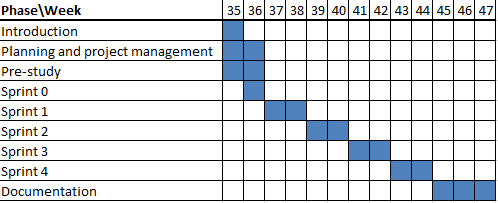
\includegraphics[width=1.0\textwidth]{project_management/project_effort_estimation}
  \caption[Gantt chart of project phases]{Gantt chart showing project phases, and when they are planned done.}
  \label{gantt:project}
\end{figure}
First week for this project is planed as an introductory week, where team members will get introduced to each other and get familiar with the project and following assignments.
After that, the first official phase of the project will last for two weeks, and refers to planning and project management. 
During this period all administrative tasks should be finished, allowing a smooth start of the actual developing process. 
At the same time, the preliminary study will be one of the occupations for all team members. 
This should give a clear picture of available technologies, development processes and project work flow for the upcoming months.
The start of the actual development is scheduled for week 36, overlapping with the previous phase. 
The development process will consist of our "sprint zero", lasting one week, and four two-week sprints. 
At the end of sprint four, in week 44, the team should finish the application development and provide a release version to the customer.
The last three weeks are reserved for finishing the documentation, which was written throughout the whole previous phases. 
During this period, the remaining sections should be finished, the whole document thoroughly revised and prepared for the final delivery.

\subsubsection{Planning and research}

This first phase of the project consists of an introduction to the course,
planning of the project, introduction to the problem domain, getting to know
the group, requirement gathering and such. In this phase the most important
decisions about system architecture, choice of COTS (Commercial off-the-shelf) and framework, project
methodology and role distribution, will be taken. Figure~\ref{gantt:pre_imp}
shows how the work will be distributed in this time period.

\begin{figure}[h]
\centering
  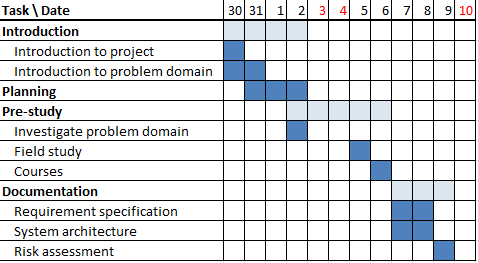
\includegraphics[width=1.0\textwidth]{project_management/pre_implementation_gantt}
  \caption[Gantt chart of planning and research phase]{Gantt diagram picturing how work should be distributed in the time available during the planning and research phase.}
  \label{gantt:pre_imp}
\end{figure}

\subsubsection{Sprints}

Each sprint will consist of four phases. Effort estimation is
detailed in Table \ref{Sprint effort estimation}.

\begin{table}[htbp]
\begin{center}
  \begin{tabular}{|r|r|r|}
    \hline
    \bf{Task} & \bf{Hours per person} & \bf{Hours total} \\
    \hline
    Planning & 8 & 56 \\
    Implementation & 8 & 56 \\
    Testing & 8 & 56 \\
    Documentation & 16 & 112 \\
    Administrative & 8 & 56 \\
    \hline \hline
    \bf{Sum} & 50 & 350 \\
    \hline
  \end{tabular}
  \caption{Task effort estimation for each sprint}
  \label{Sprint effort estimation}
\end{center}
\end{table}

\textbf{Planning} The planning phase of each sprint represents the time
required for work distribution, planning of how each task should be handled,
and how testing should be done for this section.

\textbf{Implementation} The implementation phase represents time spent on coding.
This will also include code refactoring and other maintenance tasks
related to the code.

\textbf{Testing} The testing phase represents time spent testing the system.
This includes integration testing, unit testing, functional testing etc.
The testing and implementation phases will work concurrently due to the
test-driven development methodology.

\textbf{Documentation} The documentation phase represents time spent
documenting work effort (implementation, research, etc.) and administrative
tasks like meetings.

\subsubsection{Documentation}
The last part of the project will consist of evaluating our work, and finish the documentation of the project. In addition, this part will include a final presentation November 24th for the external examiner, advisor and customer. This period will span the last three weeks of the project.  
